\documentclass{article}
\usepackage[spanish]{babel}
\usepackage[numbers,sort&compress]{natbib}
\usepackage{graphicx}
\usepackage{url}
\usepackage{amsmath}
\usepackage{hyperref}
\usepackage{float}
\usepackage{color}
\definecolor{gray86}{gray}{.86}
\definecolor{gray75}{gray}{.75}
\definecolor{gray45}{gray}{.45}
\usepackage{listings}
\lstset{ 
language=C,                
basicstyle=\footnotesize,      
numbers=left,                  
numberstyle=\footnotesize,     
stepnumber=1,                   
numbersep=5pt,                  
backgroundcolor=\color{gray86},  
showspaces=false,              
showstringspaces=false,         
showtabs=false,                
frame=single,           
tabsize=2,          
captionpos=b,          
breaklines=true,        
breakatwhitespace=false,   
escapeinside={\%*}{*)}          
}
\usepackage{subfigure} 
\usepackage[top=15mm, bottom=15mm, left=15mm, right=15mm]{geometry}
\setlength{\parskip}{2mm}
\setlength{\parindent}{0pt}

\author{Abraham Azael Morales Juárez  1422745}
\title{Frentes de Pareto}
\date{\today}

\begin{document}

\maketitle

\section{Introducción}
Un problema multicriterio es el cual tiene un conjunto de variables que le asignan valores de tal forma que se optimicen mas de 2 funciones objetivos. Aunque uno de los problemas típicos es que una función puede mejorar mientras que otra puede empeorar, además de otro tipo de restricciones que en esta práctica no se toma en cuenta\cite{REF1}. 
El generador de funciones objetivo en este caso será un generador de polinomios, estos a su vez tienen una variable por termino y un termino por variable.
Aquí es donde se toma en cuenta la dominancia de Pareto que esta es una clasificación de soluciones, es decir, si una solución domina a otra si no empeora ninguno de los objetivos y mejora a por lo menos uno\cite{REF1}.

\section{Objetivos}
Realizar una paralelización del cálculo donde convenga.\\
Graficar el porcentaje de soluciones de Pareto como función del número de funciones objetivo como diagramas de violín combinados con diagramas caja-bigote, verificando que las diferencias observadas sean estadísticamente significativas. Razona en escrito a que se debe.

\section{Resultados}
La simulación se llevó a cabo con polinomios de 5 términos, 4 variables y un grado máximo de 3, sólo se consideró 150 soluciones iniciales para buscar el porcentaje del frente de Pareto, variando de 2 hasta 10 funciones objetivos con 30 réplicas en el código en paralelo\cite{REF2}.\\
Se incluye un fragmento del código donde se observa la parte de la paralelización
\begin{lstlisting}[frame=single]
vc <- 4
md <- 3
tc <- 5
funciones <- c("pick.one", "poli", "eval", "domin.by")
variables <- c("vc", "md", "tc")
replicas <- 30

library(parallel)
mc <- makeCluster(detectCores() - 1)
clusterExport(mc, funciones)
clusterExport(mc, variables)
resultados <- data.frame(fun = integer(), rep = integer(), SolNoDom = integer(), Porcentaje = numeric())
n <- 150
for (k in 2:10) {
  clusterExport(mc, "k")
  for (r in 1:replicas) {
    
    obj <- parSapply(mc, 1:k, function(i) {
      return(list(poli(md, vc, tc)))
    })
    
    minim <- (runif(k) > 0.5)
    sign <- (-1)^minim

\end{lstlisting}
Los resultados de la simulación se observan en la figura 1, donde se observa una tendencia hacia el máximo porcentaje de 100 al momento de considerar una mayor cantidad de funciones objetivos.
\begin{figure}[H]
\centering
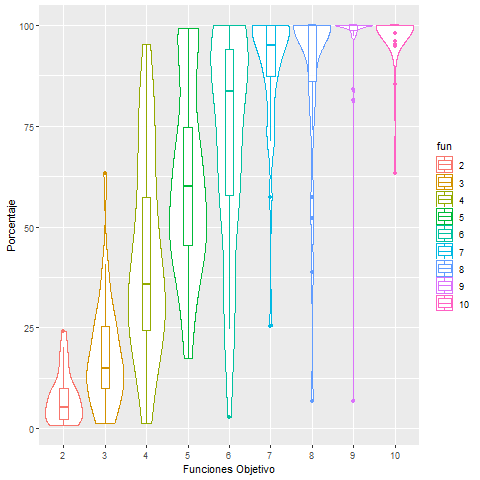
\includegraphics[width=9cm]{2.png}
\caption{Resultado de la simulación, comparando la cantidad de funciones objetivo contra el porcentaje.}
\end{figure}
También se realiza una prueba de Dunn para examinar si los datos cumplen con normalidad, con un nivel de significancia de 0.05, concluyendo que los porcentajes de soluciones no dominadas son a partir de la octava función objetivo.

También se realiza una prueba de Dunn para examinar si los datos cumplen con normalidad, figura 2.
\begin{figure}[H]
\centering
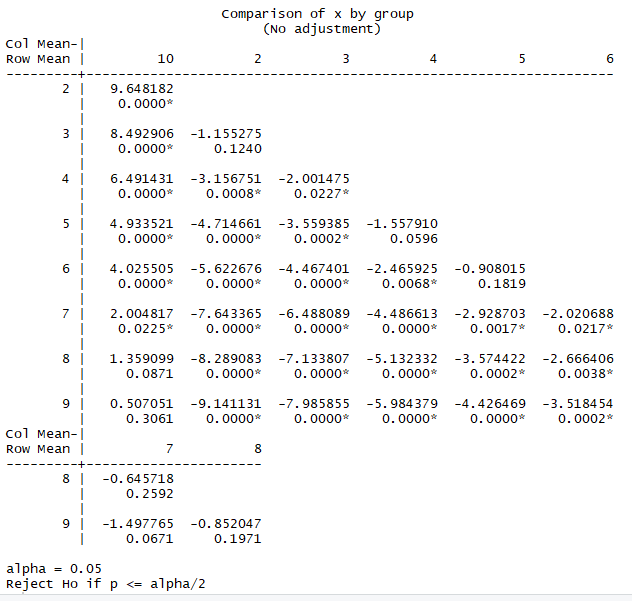
\includegraphics[width=9cm]{1.png}
\caption{Resultados de la prueba de Dunn.}
\end{figure}
También se realiza una prueba de Dunn para examinar si los datos cumplen con normalidad, con un nivel de significancia de 0.05, concluyendo que los porcentajes de soluciones no dominadas son a partir de la octava función objetivo.
\section{Conclusiones}
Se concluye que considerar 8 o una cantidad mayor de funciones objetivo no existen diferencias significativas entre los porcentajes del frente de Pareto. Mientras que de 7 o menores solo no existen diferencias significativas cuando se toman consecutivas las funciones.
\bibliographystyle{plainnat}
\bibliography{ref11}




\end{document}